% ----------------------------------------------------------
\chapter{Metodologia}\label{cap:metodologia}
% ----------------------------------------------------------

\section{Caracterização da Pesquisa}\label{sec:caracterizacao}

O presente trabalho caracteriza-se como uma pesquisa de natureza aplicada e abordagem quantitativa \cite{prodanov2013metodologia}, conduzida sobre dados secundários provenientes de um inquérito populacional de desenho transversal, no qual a exposição e o desfecho são mensurados simultaneamente \cite{rothman2008modern}. Para a condução das etapas do projeto, foi adotado o modelo \textit{Cross Industry Standard Process for Data Mining} (CRISP-DM), que, conforme evidenciado pela revisão sistemática conduzida por \textcite{schroer2021systematic}, consolida-se como o modelo de processo mais utilizado para orientar projetos de ciência de dados, mineração de dados e \textit{Machine Learning}. Em virtude de sua natureza iterativa, o modelo favorece a rastreabilidade desde a concepção do problema até a validação da solução, motivo pelo qual foi escolhido como \textit{framework} deste trabalho.

Embora a literatura aponte que o modelo original pode necessitar de adaptações de \textit{Design Thinking}\footnote{Abordagem centrada no ser humano para resolver problemas complexos e promover a inovação.} para atender a requisitos modernos de interação com o usuário final \cite{schroer2021systematic}, a robustez do CRISP-DM para o tratamento de dados estruturados torna-o adequado ao processamento dos microdados da Pesquisa Nacional de Saúde (PNS). A fim de suprir a lacuna de usabilidade apontada, a Inteligência Artificial Explicável (XAI) foi integrada ao processo por meio do método SHAP \cite{salih2025perspective}, visando proporcionar a transparência necessária à aceitabilidade do modelo no contexto da APS brasileira. Além disso, cada decisão tomada ao longo da execução e não prevista no projeto de pesquisa foi registrada juntamente com o motivo que a originou e com a sua relação com o projeto, de maneira que o percurso metodológico pudesse ser auditado, conforme descrito no capítulo de Desenvolvimento.

\section{Considerações Éticas}

Para o desenvolvimento deste trabalho, foram utilizados exclusivamente microdados públicos e anonimizados, disponibilizados pelo Instituto Brasileiro de Geografia e Estatística (IBGE) por meio da Subamostra Laboratorial da Pesquisa Nacional de Saúde de 2013 \cite{IBGE_PNS2013_Exames}. A Resolução CNS nº 466/2012 estabelece as diretrizes gerais para as pesquisas envolvendo seres humanos, definindo-as de forma a incluir o manejo de seus dados, e remete a uma resolução complementar as especificidades das pesquisas que se utilizam de metodologias próprias das ciências humanas e sociais \cite{brasil2012resolucao466}, papel exercido pela Resolução CNS nº 510/2016. Diante disso, em virtude da natureza secundária dos dados e da impossibilidade de identificação individual dos participantes, a pesquisa dispensou a submissão e a aprovação por Comitê de Ética em Pesquisa (CEP), conforme o artigo 1º, parágrafo único, incisos II e III, da Resolução CNS nº 510/2016, que excluem do registro e da avaliação pelo sistema CEP/CONEP as pesquisas que utilizam informações de acesso público e de domínio público \cite{cns2016resolucao510}. A íntegra das duas resoluções é apresentada nos Anexos~\ref{anexo:res510} e~\ref{anexo:res466}.

\section{Base de Dados e Amostra Analítica}\label{sec:base-dados}

A escolha da Pesquisa Nacional de Saúde (PNS) de 2013, em detrimento da edição de 2019, deu-se em virtude de uma diferença metodológica decisiva entre as duas pesquisas, visto que somente a edição de 2013 contou com a Subamostra Laboratorial, na qual foram coletados exames de Hemoglobina Glicada (HbA1c)\footnote{Exame de sangue que mede a média dos níveis de glicose no sangue nos últimos dois a três meses, essencial para o diagnóstico e controle do diabetes.} de 8.952 participantes adultos \cite{IBGE_PNS2013_Exames}. Por meio desta variável laboratorial, o presente trabalho viabilizou um desfecho clínico objetivo (HbA1c $\geq$ 6,5\%) como referência para o modelo, em substituição ao diagnóstico autorreferido, abordagem reconhecida pela literatura como suscetível a vieses de subnotificação na população brasileira \cite{muzy2021prevalencia,reis2022evolution,deAlmeida-Pititto09112015}. Diante disso, a edição de 2013 ofereceu o suporte necessário à premissa central do trabalho, a qual preconiza a utilização de dados clínicos objetivos como critério superior ao autorrelato para a classificação de perfis associados à hiperglicemia crônica.

A partir dos microdados, a amostra analítica foi construída por meio de critérios de exclusão aplicados registro a registro, ou seja, sem o uso de qualquer estatística calculada sobre o conjunto de dados, a fim de que nenhuma informação dos registros posteriormente destinados ao teste influenciasse a construção da amostra. Foram excluídos os registros duplicados; os registros sem valor válido de HbA1c, visto que a estimação da variável-alvo comprometeria a validade do desfecho modelado; e os registros sem nenhuma das medidas do bloco de aferição física, composto por peso, altura, circunferência da cintura e pressões arteriais sistólica e diastólica. Além disso, o código correspondente à categoria ignorada da variável raça/cor foi tratado como valor ausente, de maneira que esse código fosse imputado juntamente com os demais valores ausentes. Por fim, o desfecho foi binarizado no ponto de corte de HbA1c $\geq$ 6,5\%, conforme o critério diagnóstico da \textcite{ADA2010}. A caracterização numérica da amostra resultante é apresentada no capítulo de Resultados.

Em virtude do desenho amostral complexo da PNS 2013, o IBGE disponibiliza o peso amostral laboratorial (\textit{Peso\_Lab}), cuja função é corrigir as estimativas de parâmetros populacionais, como taxas e proporções, para a população adulta brasileira \cite{IBGE}. No presente trabalho, o \textit{Peso\_Lab} foi utilizado exclusivamente na etapa descritiva, na estimação da prevalência ponderada do desfecho, e não foi fornecido a nenhum dos algoritmos durante o treinamento. Essa distinção decorre da diferença entre os dois objetivos, visto que a ponderação amostral corrige a estimativa de um parâmetro da população, enquanto o modelo classificatório tem como objetivo ordenar indivíduos segundo a associação de suas características com o desfecho, tarefa na qual cada registro representa a si mesmo, e não a parcela da população que o peso lhe atribui. Diante disso, o argumento que motivou a rejeição do SMOTE, apresentado no referencial teórico, permanece coerente com esta decisão, já que a preservação dos registros originais é o que mantém válidas as estimativas ponderadas produzidas na etapa descritiva.

\section{Estrutura do Pipeline CRISP-DM}\label{sec:pipeline-crisp}

Conforme ilustrado na Figura \ref{fig:ciclodevida}, o modelo CRISP-DM possui um ciclo de vida de seis fases iterativas \cite{wirth2000crisp}, o qual foi seguido pelo presente trabalho e adaptado ao contexto do sistema público de saúde brasileiro, conforme descrito a seguir.
\begin{figure}[H]
    \centering
    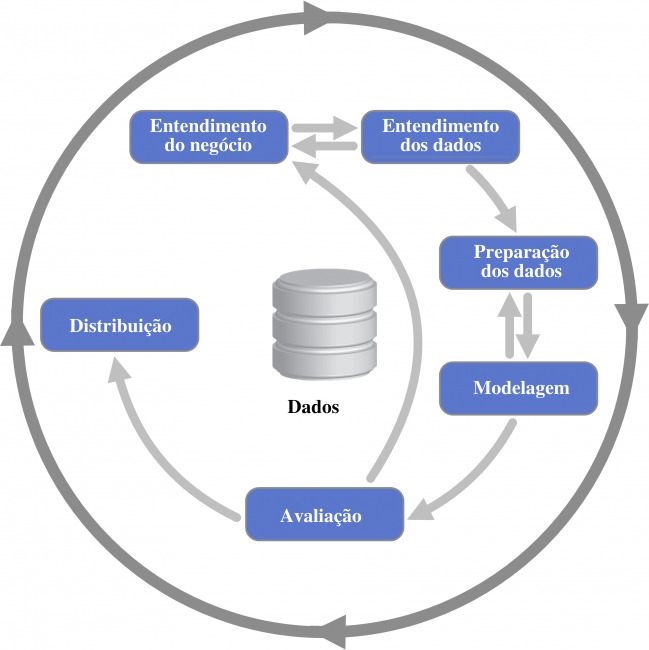
\includegraphics[scale=0.35]{figs/Ciclo de vida CRISP-DM.png}
    \caption{Ciclo de vida CRISP-DM.}
    \label{fig:ciclodevida}
\end{figure}

\begin{enumerate}
    \item \textbf{Compreensão do Negócio (\textit{Business Understanding}):} Nesta fase inicial, o foco consiste em compreender os objetivos e requisitos sob uma perspectiva operacional \cite{wirth2000crisp}. O conhecimento adquirido foi convertido em um problema formal de mineração de dados, ou seja, o desenvolvimento de um modelo de classificação supervisionado que utiliza os microdados da Subamostra Laboratorial da PNS 2013 \cite{IBGE_PNS2013_Exames}, cuja função é identificar indivíduos com perfis associados à hiperglicemia crônica clinicamente significativa, definida pelo critério laboratorial de HbA1c $\geq$ 6,5\%, conforme a reformulação conceitual do desfecho apresentada ao final desta seção.

    \item \textbf{Compreensão dos Dados (\textit{Data Understanding}):} Nesta fase, foi realizada a extração dos microdados da Subamostra Laboratorial da Pesquisa Nacional de Saúde, seguida de uma Análise Exploratória de Dados (EDA), a fim de mapear a distribuição das variáveis sociodemográficas, antropométricas e biológicas \cite{morgenthaler2009exploratory}, identificar correlações entre as variáveis e quantificar os valores ausentes e as anomalias presentes na amostra \cite{sahoo2019exploratory}. Na etapa descritiva, a prevalência do desfecho foi estimada também de forma ponderada pelo \textit{Peso\_Lab}, conforme descrito na seção de Base de Dados e Amostra Analítica. Os achados desta etapa subsidiaram as decisões sobre a seleção das variáveis de classificação e sobre o tratamento dos valores ausentes.

   \item \textbf{Preparação dos Dados (\textit{Data Preparation}):} Com base na análise exploratória, os dados foram submetidos a um \textit{pipeline} sequencial de preparação, estruturado a fim de prevenir qualquer forma de vazamento de informação (\textit{data leakage}) entre os subconjuntos de treino e teste. Inicialmente, o conjunto de dados foi dividido em treino (80\%) e teste (20\%), preservando a proporção da variável-alvo nos dois subconjuntos. Todas as etapas que aprendem parâmetros a partir dos dados, como a imputação de valores ausentes por meio do algoritmo \textit{K-Nearest Neighbors} (KNN) e a padronização das variáveis contínuas, foram ajustadas exclusivamente sobre o conjunto de treino e posteriormente aplicadas ao conjunto de teste, evitando assim a contaminação deste \cite{pedregosa2011scikit}. O detalhamento destas etapas é apresentado na seção de Preparação dos Dados, e o tratamento do desbalanceamento de classes, realizado por meio de aprendizagem sensível ao custo (\textit{Cost-Sensitive Learning}), é apresentado na seção de Tratamento do Desbalanceamento.

    \item \textbf{Modelagem (\textit{Modeling}):} Os microdados processados serviram de base para o treinamento de dois algoritmos de classificação supervisionada, implementados por meio da linguagem Python e da biblioteca \textit{scikit-learn} \cite{pedregosa2011scikit}. O primeiro algoritmo foi a Regressão Logística, utilizada como \textit{baseline} interpretável em virtude de sua transparência paramétrica e da consolidação histórica em estudos epidemiológicos \cite{nusinovici2020logistic}. O segundo foi o \textit{Random Forest}, escolhido em virtude de sua robustez frente à presença de variáveis correlacionadas, de sua capacidade de modelar interações não lineares entre as variáveis e de sua compatibilidade com técnicas de explicabilidade baseadas em valores de Shapley \cite{salih2025perspective}, cujos hiperparâmetros foram definidos por meio de uma busca descrita na seção de Modelagem. Seguindo o fluxo iterativo do CRISP-DM \cite{wirth2000crisp}, os achados desta fase motivaram retornos à fase de preparação dos dados, a exemplo do diagnóstico de multicolinearidade, que levou à remoção de uma variável e ao descarte de um dos conjuntos de atributos avaliados.

    \item \textbf{Avaliação (\textit{Evaluation}):} Os modelos desenvolvidos foram submetidos a um protocolo de avaliação em duas etapas. No conjunto de treino, a Validação Cruzada Estratificada com $k = 5$ \textit{folds} \cite{pertiwi2020comparison} foi utilizada para definir o limiar de decisão de cada modelo e para medir a variação das métricas entre partições \cite{pedregosa2011scikit}. No conjunto de teste, os modelos foram avaliados por meio de métricas derivadas da Matriz de Confusão \cite{Swaminathan2024}, tendo a Sensibilidade (\textit{Recall}) como métrica prioritária em virtude do contexto clínico de triagem, acompanhada da Especificidade, do \textit{F1-Score} e da Área Sob a Curva ROC (AUC-ROC) \cite{fawcett2006introduction, powers2020evaluation}. A essas métricas, previstas no projeto de pesquisa, somaram-se métricas complementares, a calibração das probabilidades e a comparação com uma regra clínica de rastreamento, de maneira que fosse possível identificar a estratégia mais adequada à tarefa de triagem proposta. O protocolo completo é apresentado na seção de Avaliação.

   \item \textbf{Implantação (\textit{Deployment}):} A fase de implantação compreende o painel de resultados, desenvolvido por meio do \textit{framework} Streamlit, e a disponibilização do modelo de referência por meio de uma API construída com o \textit{framework} FastAPI \cite{ramirez2018fastapi}, ambos descritos no capítulo de Desenvolvimento.
\end{enumerate}

\subsection{Reformulação Conceitual do Desfecho}
Para a operacionalização do desfecho do presente trabalho, fez-se necessária uma redefinição conceitual a partir das limitações intrínsecas da base de dados utilizada. A Subamostra Laboratorial da Pesquisa Nacional de Saúde (PNS) de 2013 não disponibiliza variável que diferencie clinicamente o Diabetes Mellitus tipo 1 (DM1) do tipo 2 (DM2), visto que o critério diagnóstico laboratorial de Hemoglobina Glicada (HbA1c) $\geq 6,5$\%, estabelecido pela American Diabetes Association \cite{ADA2010}, identifica a presença de hiperglicemia crônica independentemente do mecanismo patogênico subjacente.
Diante disso, o desfecho modelado por esta pesquisa foi reformulado como a presença de hiperglicemia crônica clinicamente significativa em adultos, operacionalizada por HbA1c $\geq$ 6,5\%, em detrimento da tentativa de discriminação diagnóstica entre subtipos de DM. Essa decisão metodológica sustenta-se em quatro fundamentos.
Em primeiro lugar, a literatura epidemiológica internacional indica que, entre adultos com diagnóstico de diabetes, mais de 90\% dos casos correspondem ao DM2 \cite{who2024diabetes}. No escopo nacional, o cenário não é diferente, visto que, segundo o Ministério da Saúde, cerca de 90\% dos pacientes diabéticos no Brasil possuem DM2 \cite{brasil2024diabetes}.

Em segundo lugar, no contexto da APS, a função do mecanismo de triagem proposto não consiste na discriminação diferencial entre subtipos de diabetes, mas sim na identificação precoce de indivíduos com perfis associados à hiperglicemia clinicamente significativa, gerando, por consequência, o encaminhamento para investigação laboratorial complementar \cite{brasil2013}. Logo, a responsabilidade da classificação etiológica específica é alocada à etapa subsequente do fluxo assistencial, conduzida por profissional médico em âmbito especializado.

Em terceiro lugar, as variáveis operacionalizadas pelo modelo correspondem predominantemente a determinantes associados ao DM2, tanto de natureza biológica, como a idade, a adiposidade e a hipertensão arterial sistêmica \cite{mlynarska2025type}, quanto de natureza social, como a escolaridade e a região \cite{deAlmeida-Pititto09112015}. Diante disso, os casos residuais de DM1 presentes na subamostra atuam como ruído no rótulo do desfecho, cuja proporção é limitada pela própria distribuição dos subtipos da doença, visto que cerca de 90\% dos casos de diabetes correspondem ao DM2 \cite{who2024diabetes, brasil2024diabetes}. Logo, admite-se que esse ruído, por representar uma fração minoritária dos casos positivos, não altera de forma expressiva as associações aprendidas pelos algoritmos, sendo este um pressuposto do presente trabalho e não uma garantia demonstrada empiricamente.

Em quarto lugar, há precedente direto na literatura que utiliza a própria PNS 2013 com critério laboratorial, visto que \textcite{muzy2021prevalencia}, ao estimar a prevalência de diabetes a partir da HbA1c da Subamostra Laboratorial, assumiram que a totalidade dos casos correspondia ao DM2, em virtude de 90\% a 95\% dos casos de diabetes serem desse tipo, corroborando a reformulação adotada neste trabalho.

\section{Seleção de Variáveis}\label{sec:selecao-variaveis}

\subsection{Princípios Orientadores}\label{sec:principios}
A seleção do conjunto de variáveis de classificação foi conduzida a partir de quatro princípios norteadores, estabelecidos com o objetivo de garantir a viabilidade científica, clínica e operacional do modelo proposto.

Pelo primeiro princípio, de não invasividade, foi priorizada a seleção exclusiva de variáveis obtidas por meio de entrevista, medição antropométrica ou aferição clínica não invasiva, a fim de viabilizar a aplicação do modelo no contexto da APS, no qual procedimentos laboratoriais representam, muitas vezes, barreiras estruturais e financeiras para a triagem populacional sistemática \cite{geremia2020atenccao}.

O segundo princípio, de compatibilidade com os sistemas de informação existentes, restringiu a composição do conjunto final às variáveis rotineiramente capturadas pelo Prontuário Eletrônico do Cidadão (PEC) no âmbito do Sistema de Informação em Saúde para a Atenção Básica (SISAB) \cite{brasil_esus_aps}, de maneira que, em trabalhos futuros, a metodologia desenvolvida apresente potencial de integração às bases de dados já consolidadas na rede pública brasileira sem exigência de coleta de novos dados ou alteração expressiva do fluxo assistencial.

O terceiro princípio, de robustez contra causalidade reversa, foi particularmente sensível em virtude da natureza transversal da PNS 2013 \cite{rothman2008modern}. Variáveis comportamentais estão sujeitas a alteração sistemática pós-diagnóstico de diabetes \cite{dimova2020diagnosis}, em especial a prática de exercício físico e o padrão alimentar, visto que as orientações clínicas posteriores ao diagnóstico prescrevem a inclusão ou o aumento da atividade física e a melhora da alimentação \cite{brasil2013}. Essas variáveis foram deliberadamente excluídas do conjunto final, a fim de mitigar a introdução de vieses de causalidade reversa no processo de aprendizagem do algoritmo. Caso mantidas, tais variáveis poderiam induzir o modelo a aprender regras estatisticamente invertidas, nas quais a presença de comportamento saudável se associa positivamente à condição patológica.

O quarto princípio, de parcimônia estatística e interpretabilidade, orientou a priorização de variáveis conceitualmente ortogonais, evitando redundância excessiva que dilua a interpretabilidade das contribuições individuais via SHAP (SHapley Additive exPlanations), cuja função é proporcionar a visualização do peso relativo de cada variável na classificação individual realizada pelo modelo \cite{salih2025perspective}.

\subsection{Variáveis Candidatas}\label{sec:variaveis-candidatas}
O conjunto de variáveis candidatas é composto por dezesseis variáveis, sendo quatorze obtidas diretamente dos microdados ou derivadas registro a registro e duas compostas, organizadas em cinco blocos temáticos, conforme apresentado a seguir. A composição de cada conjunto de atributos efetivamente utilizado no treinamento, a partir dessas candidatas, é apresentada na subseção de Conjuntos de Atributos.

Os códigos alfanuméricos dispostos entre parênteses ao longo desta seção, exemplo (C008), (Z001) e (W00303), correspondem aos identificadores oficiais de cada variável presentes no dicionário de microdados da Subamostra Laboratorial da Pesquisa Nacional de Saúde (PNS) de 2013, disponibilizado pelo IBGE \cite{IBGE_PNS2013_Exames}. A sua inclusão tem como objetivo viabilizar a rastreabilidade e a reprodutibilidade do estudo, de maneira que pesquisadores que venham a utilizar a mesma base de dados possam localizar com precisão cada variável operacionalizada no presente trabalho.

\begin{itemize}
\item[] \textbf{Variáveis Antropométricas e Biológicas: }
A inclusão das variáveis idade (C008) e sexo (Z001) fez-se necessária em virtude do papel determinante do envelhecimento na deterioração funcional das células beta pancreáticas e da sarcopenia progressiva \cite{mlynarska2025type}, bem como da prevalência diferenciada do DM2 entre sexos constatada em estudos populacionais brasileiros \cite{deAlmeida-Pititto09112015,muzy2021prevalencia,reis2022evolution}. O Índice de Massa Corporal (IMC) foi computado como variável derivada a partir da razão entre o peso final (z004) e o quadrado da altura final (z005), seguindo a fórmula clássica de Quetelet, cuja função é abranger a magnitude geral do acúmulo de tecido adiposo como indicador basal de resistência à insulina \cite{mlynarska2025type}. O peso e a altura foram utilizados apenas no cálculo das variáveis derivadas, não sendo fornecidos diretamente aos algoritmos, a fim de evitar que a mesma informação entrasse no modelo por canais redundantes.

A Circunferência da Cintura (W00303) foi incorporada em virtude da superioridade classificatória da adiposidade visceral sobre a adiposidade subcutânea generalizada, conforme fundamentado no referencial teórico. Diante disso, a utilização isolada do IMC como critério de triagem configura-se insuficiente para a identificação de perfis de risco metabólico relevantes na população adulta, de maneira que a mensuração complementar da circunferência da cintura torna-se necessária para a classificação dos perfis. A aferição desta variável na Subamostra Laboratorial da PNS 2013 seguiu o protocolo padronizado pelo IBGE, segundo o qual a medição foi realizada no ponto médio entre a borda inferior da última costela e a borda superior da crista ilíaca \cite{ibge2013pns}. A manutenção dessa variável em sua forma absoluta, mensurada em centímetros, se justifica pela existência de pontos de corte clinicamente consolidados para esse protocolo de aferição específico (circunferência $\geq 80$ cm para mulheres e $\geq 94$ cm para homens) \cite{SBD2019}.

Complementarmente, a Razão Cintura-Estatura (RCEst), derivada a partir da divisão entre Circunferência da Cintura (W00303) e altura final (z005), foi incluída como variável auxiliar, cujo papel é capturar a adiposidade visceral ajustada pela estatura individual, dimensão que não é abrangida de forma integral pelo IMC ou pela CC absoluta isoladamente \cite{Feller2010}. Diante disso, o bloco antropométrico candidato reúne três variáveis complementares sobre o fenótipo corporal do indivíduo, cuja permanência no modelo final foi condicionada ao diagnóstico descrito na seção de Tratamento da Multicolinearidade.

\item[] \textbf{Variáveis de Pressão Arterial Sistêmica: }
A Pressão Arterial Sistólica (W00407) e a Pressão Arterial Diastólica (W00408) foram incorporadas em suas formas contínuas aferidas objetivamente durante a coleta da PNS 2013 \cite{ibge2013pns}. A inclusão das medidas objetivas, em detrimento do uso exclusivo do autorrelato de HAS, é metodologicamente coerente com a premissa central deste trabalho, a qual preconiza a utilização de dados objetivos como critério superior ao autorrelato, em razão do fenômeno amplamente documentado de subnotificação diagnóstica na população brasileira \cite{muzy2021prevalencia,reis2022evolution,deAlmeida-Pititto09112015}.
 Adicionalmente, a variável HAS autorrelatada (Q002) foi mantida, com o objetivo de capturar a dimensão de consciência diagnóstica do indivíduo, variável esta que se comporta como proxy de acesso prévio ao sistema de saúde e de letramento em saúde. A partir da combinação destas duas fontes de informação, foi construída a variável derivada HAS Combinada, operacionalizada como positiva quando a pressão sistólica aferida é igual ou superior a 140 mmHg ou a diastólica é igual ou superior a 90 mmHg, conforme as diretrizes da Sociedade Brasileira de Diabetes \cite{SBD2019}, ou quando o autorrelato de diagnóstico é afirmativo, desconsiderando-se o relato de hipertensão exclusivamente durante a gravidez, de maneira que o modelo possa abranger tanto hipertensos previamente diagnosticados quanto hipertensos não diagnosticados, característica relevante para uma ferramenta de triagem que visa justamente identificar indivíduos em situação de vulnerabilidade clínica oculta.

\item[] \textbf{Diagnósticos Prévios Autorrelatados: }
O diagnóstico autorrelatado de colesterol alto (Q060) foi incorporado em virtude do papel consolidado da dislipidemia na Síndrome Metabólica, conforme fundamentado no referencial teórico.
Adicionalmente, foi desenvolvida a variável derivada \textit{Multimorbidade Metabólica}, operacionalizada como escore ordinal de zero a três, a partir da soma de três condições clínicas: HAS Combinada positiva; autorrelato afirmativo de colesterol alto (Q060); e presença de obesidade, definida pela ocorrência de IMC $\geq$ 30 kg/m² ou de Circunferência da Cintura $\geq$ 80 cm em mulheres ou $\geq$ 94 cm em homens \cite{SBD2019}. 
A escolha pela operacionalização disjuntiva do componente de obesidade, de maneira que a evidência por qualquer um dos dois indicadores antropométricos seja suficiente para a ativação do componente, fez-se necessária em virtude da limitação reconhecida do IMC isolado para a identificação de adiposidade central, conforme evidenciado na literatura \cite{Feller2010}.
O agrupamento de comorbidades metabólicas em um escore único busca viabilizar a captura de interações sinérgicas entre condições clínicas que, isoladamente, poderiam não atingir o limiar identificável pelos algoritmos, mas que, conforme a literatura especializada, em combinação elevam expressivamente a probabilidade de hiperglicemia crônica clinicamente significativa \cite{SBD2019,rzewuska2017epidemiology}.

\item[] \textbf{Variáveis Sociodemográficas: }
A raça/cor (Z003), a escolaridade (VDD004) e a posse de plano de saúde (I001) foram incorporadas como determinantes sociais da saúde, visto que, conforme o levantamento bibliográfico, estas variáveis atuam como \textit{proxies} das iniquidades históricas, do letramento em saúde e do acesso diferencial à rede assistencial brasileira \cite{deAlmeida-Pititto09112015,muzy2021prevalencia,reis2022evolution}. A raça/cor, em particular, foi interpretada neste trabalho exclusivamente como marcador de determinação social e de acesso aos serviços de saúde, e não como variável biológica.
A variável região (regiao) abrange a dimensão da heterogeneidade territorial brasileira, visto que a literatura constatou disparidades expressivas na prevalência e na subnotificação do DM2 entre as cinco macrorregiões do país \cite{muzy2021prevalencia,deAlmeida-Pititto09112015,reis2022evolution}.

\item[] \textbf{Autopercepção de Saúde: }
O estado de saúde autoavaliado (N001) foi mantido no conjunto final apesar de sua natureza subjetiva, em virtude da consolidação desta variável como indicador associado a desfechos crônicos em estudos epidemiológicos transversais e longitudinais, conforme descrito no referencial teórico \cite{Rantanen2019}. 
\end{itemize}

\subsection{Conjuntos de Atributos}\label{sec:conjuntos-atributos}
A partir das variáveis candidatas, foram construídos três conjuntos de atributos, cuja função é avaliar, por meio de experimentação, o efeito da redundância entre variáveis sobre o desempenho e a interpretabilidade dos modelos, em conformidade com o protocolo de tratamento da multicolinearidade previsto no projeto de pesquisa e com o quarto princípio orientador da seleção de variáveis. A composição de cada conjunto é apresentada no Quadro~\ref{qua:conjuntos}.

\begin{quadro}[htb]
  \caption{\label{qua:conjuntos}Conjuntos de atributos avaliados.}
  \small
  \begin{tabular}{|p{2.2cm}|p{6.2cm}|c|p{4.2cm}|}
    \hline
    \textbf{Conjunto} & \textbf{Variáveis} & \textbf{Colunas} & \textbf{Papel} \\ \hline
    A, atômico & Idade, IMC, CC, PAS, PAD, escolaridade, autopercepção de saúde, sexo, plano de saúde, raça/cor, região, HAS autorrelatada e colesterol alto & 20 & Componentes isolados, sem escores agregados \\ \hline
    B, composto & Idade, IMC, CC, escolaridade, autopercepção de saúde, Multimorbidade Metabólica, sexo, plano de saúde, raça/cor e região & 16 & Escore de multimorbidade no lugar das pressões e dos diagnósticos autorrelatados \\ \hline
    C, completo & As dezesseis candidatas, incluindo RCEst, HAS Combinada e Multimorbidade Metabólica & 23 & Componentes e escores simultaneamente \\ \hline
  \end{tabular}
  \fonte{Elaborado pelo autor.}
\end{quadro}

Na coluna ``Colunas'', considera-se o número de colunas da matriz de dados fornecida aos algoritmos, após a codificação das variáveis nominais. A diferença entre os conjuntos reside no grau de ortogonalidade entre essas colunas, avaliado em dois níveis. No nível estrito, nenhuma variável de origem entra no modelo, ao mesmo tempo, como coluna própria e como parcela idêntica de uma variável agregada, condição atendida pelos conjuntos A e B. No nível pleno, nenhuma variável de origem contribui para o modelo por mais de um caminho, em qualquer forma, condição atendida apenas pelo conjunto A. Esses dois níveis foram verificados por testes automatizados sobre a proveniência de cada coluna, descritos no capítulo de Desenvolvimento.

No conjunto B, permanece uma sobreposição residual, visto que o IMC, a circunferência da cintura e o sexo entram como colunas próprias e também alimentam o componente de obesidade do escore de multimorbidade, porém em forma binarizada por ponto de corte clínico, de maneira que o gradiente contínuo dessas variáveis carrega uma informação que o limiar descarta. Pelo mesmo motivo de ortogonalidade, a HAS Combinada, que constitui a primeira parcela do escore, foi mantida fora do conjunto B, a fim de que o modelo não recuperasse a parcela diretamente e a hipótese de sinergia entre as condições clínicas permanecesse testável. Já o conjunto C repete deliberadamente a mesma informação por mais de um canal, a exemplo da HAS autorrelatada e do colesterol alto, que entram como colunas próprias e novamente dentro do escore, com o objetivo de quantificar o custo dessa redundância. Por fim, a RCEst integra apenas o conjunto C, visto que sua exclusão dos conjuntos A e B decorreu do diagnóstico descrito na seção de Tratamento da Multicolinearidade, cujos valores são apresentados no capítulo de Resultados.

\section{Preparação dos Dados}\label{sec:preparacao}

\subsection{Particionamento}\label{sec:particionamento}
A amostra analítica foi dividida em um conjunto de treino, com 80\% dos registros, e um conjunto de teste, com os 20\% restantes, por meio de amostragem estratificada pela variável-alvo, de maneira que a proporção de casos positivos fosse preservada nos dois subconjuntos \cite{pedregosa2011scikit}. Nenhuma operação que dependesse de mais de um registro foi executada antes dessa divisão, a fim de que nenhuma informação do conjunto de teste influenciasse qualquer etapa do treinamento. Diante disso, toda etapa que aprende parâmetros a partir dos dados, como a imputação, a padronização e a codificação das variáveis, foi ajustada exclusivamente sobre o conjunto de treino e apenas aplicada ao conjunto de teste. Todas as operações estocásticas do trabalho, incluindo a divisão dos dados, utilizaram a mesma semente aleatória, de valor 42, a fim de garantir a reprodutibilidade dos resultados.

\subsection{Imputação de Valores Ausentes}\label{sec:imputacao}
Os valores ausentes das variáveis classificadoras foram imputados por meio do algoritmo \textit{K-Nearest Neighbors} (KNN), conforme previsto no projeto de pesquisa, utilizando cinco vizinhos ponderados pelo inverso da distância \cite{pedregosa2011scikit}. A variável-alvo não foi imputada, visto que os registros sem valor válido de HbA1c já haviam sido excluídos da amostra analítica. A imputação foi posicionada como a primeira etapa do \textit{pipeline} de preparação e aplicada sobre todas as variáveis candidatas, e não apenas sobre as colunas de cada conjunto de atributos, em virtude de as variáveis compostas, construídas na etapa seguinte, dependerem de componentes que nem todos os conjuntos utilizam como coluna própria.

Como o KNN seleciona os vizinhos por meio da distância euclidiana, a aplicação direta do algoritmo sobre as variáveis em suas escalas originais faria com que as variáveis de maior amplitude numérica, como a pressão arterial e a idade, dominassem a seleção dos vizinhos. Diante disso, o espaço de distância foi restrito às variáveis contínuas, padronizadas por meio de um ajuste realizado apenas sobre o conjunto de treino, e à variável sexo, por ser binária e, portanto, a única variável categórica em que a distância possui significado direto. As demais variáveis categóricas, como raça/cor, região e escolaridade, não participaram do cálculo da distância, visto que a diferença numérica entre seus códigos não representa uma diferença real entre categorias, porém permaneceram como alvo da imputação. Os valores imputados dessas variáveis foram arredondados para o código válido mais próximo entre os observados no treino, de maneira que a codificação posterior permanecesse consistente. Por fim, as variáveis contínuas foram devolvidas à sua escala clínica original após a imputação, visto que as variáveis compostas utilizam pontos de corte expressos em unidades reais.

\subsection{Variáveis Derivadas}\label{sec:derivadas}
As variáveis derivadas foram construídas em dois momentos distintos, conforme dependessem ou não de informações de outros registros. O IMC, calculado pela razão entre o peso em quilogramas e o quadrado da altura em metros, e a RCEst, calculada pela razão entre a circunferência da cintura e a altura, foram construídos registro a registro durante a limpeza dos dados, visto que dependem apenas das medidas do próprio indivíduo. Já as variáveis compostas, isto é, a HAS Combinada e a Multimorbidade Metabólica, foram construídas dentro do \textit{pipeline}, após a imputação, em virtude de dependerem de componentes imputados, cujo ajuste é realizado apenas sobre o conjunto de treino. A construção dessas variáveis antes da divisão dos dados faria com que o conjunto de teste carregasse uma imputação ajustada sobre a base completa, configurando vazamento de informação. Nesta mesma etapa, as variáveis sexo, posse de plano de saúde e colesterol alto foram recodificadas como indicadoras binárias.

Na última etapa do \textit{pipeline}, cada conjunto de atributos selecionou as suas colunas, sobre as quais foram aplicadas a padronização das variáveis numéricas, a manutenção das variáveis binárias em sua forma original e a codificação das variáveis nominais em variáveis indicadoras, omitindo-se uma categoria de referência por variável \cite{pedregosa2011scikit}. Por consequência dessa omissão, a categoria de referência de cada variável nominal não possui coluna própria, característica que influencia a leitura da explicabilidade, conforme descrito na seção de Explicabilidade.

\section{Tratamento da Multicolinearidade}\label{sec:trat-multicolinearidade}

A manutenção simultânea de variáveis antropométricas correlacionadas (IMC, CC e RCEst) e de múltiplas variáveis de pressão arterial configurou um cenário de multicolinearidade que demandou tratamento metodológico específico, conforme apresentado no referencial teórico. A fim de diagnosticar esse problema, foram computados, sobre o conjunto de treino, os coeficientes de correlação de Pearson entre as variáveis contínuas e os Fatores de Inflação de Variância (VIF) de cada coluna \cite{Senaviratna2019}. O VIF foi calculado sobre a matriz de dados completa fornecida aos algoritmos, isto é, após a padronização e a codificação das variáveis nominais, de maneira que as variáveis binárias e as indicadoras também fossem incluídas no diagnóstico. Ao lado de cada VIF, foi reportado o coeficiente de determinação ($R^2$) da regressão auxiliar correspondente, obtido por $R^2 = 1 - 1/\text{VIF}$, visto que este expressa diretamente a fração da variância de uma coluna já explicada pelas demais.

O protocolo foi orientado pelo limiar convencional de VIF $> 10$ \cite{Senaviratna2019}. Para as variáveis de um mesmo bloco temático que excederam esse limiar, a variável de maior VIF foi removida de forma experimental e o diagnóstico foi recalculado, a fim de verificar se a remoção resolvia a violação ou se a redundância persistia nas demais colunas. No que se refere ao \textit{Random Forest}, a multicolinearidade não compromete o desempenho classificatório do algoritmo \cite{Chan2022}, de maneira que o tratamento nesse modelo foi direcionado ao plano da interpretabilidade, conforme descrito na seção de Explicabilidade.

Adicionalmente, a redundância entre o escore de Multimorbidade Metabólica e os seus componentes foi avaliada por um teste complementar ao VIF. Como o escore é obtido pela soma de três parcelas, das quais uma, o componente de obesidade, decorre da aplicação de pontos de corte sobre o IMC e a circunferência da cintura, a dependência entre o escore e as colunas contínuas não é linear e não pode ser integralmente capturada pela regressão auxiliar do VIF. Diante disso, o escore foi regredido diretamente sobre as suas três parcelas, de maneira que um coeficiente de determinação igual a um indicasse que o escore não acrescenta nenhuma informação ausente de seus componentes. Este teste não estava previsto no projeto de pesquisa e foi acrescentado em virtude dessa limitação estrutural do VIF diante de variáveis construídas por ponto de corte.

\section{Tratamento do Desbalanceamento}\label{sec:desbalanceamento}

Em virtude da baixa prevalência do desfecho na amostra, o desbalanceamento entre as classes foi tratado por meio de aprendizagem sensível ao custo, conforme previsto no projeto de pesquisa, em detrimento de técnicas de reamostragem como o SMOTE, cuja geração de observações sintéticas é incompatível com a estrutura de ponderação amostral da PNS 2013, conforme discutido no referencial teórico \cite{araf2024costsensitive, 10.1371/journal.pone.0280387}. Nenhum registro foi criado, removido ou duplicado para equilibrar as classes, visto que a estratégia adotada atua sobre a função de perda dos algoritmos, atribuindo maior peso aos erros de classificação da classe minoritária.

Na Regressão Logística, essa estratégia foi implementada por meio do hiperparâmetro \texttt{class\_weight='balanced'}, que atribui a cada classe um peso inversamente proporcional à sua frequência no conjunto de treino \cite{pedregosa2011scikit}. No \textit{Random Forest}, foi utilizada a variante \texttt{class\_weight='balanced\_subsample'}, na qual o mesmo cálculo é refeito sobre a amostra \textit{bootstrap} de cada árvore \cite{sklearn2026randomforest}. A atribuição de pesos distintos por classe em florestas aleatórias é uma abordagem estudada para o processamento de dados médicos desbalanceados, com melhora na identificação da classe minoritária \cite{zhu2018classweights}.

O projeto de pesquisa nomeava literalmente o valor \texttt{balanced} para os dois algoritmos, de maneira que a adoção da variante por subamostra na floresta constitui uma divergência formal em relação ao texto assinado, porém não em relação ao método nele estabelecido, visto que ambos os valores implementam a aprendizagem sensível ao custo e nenhum deles cria observações sintéticas. A diferença reside no fato de que, em uma floresta, cada árvore é ajustada sobre uma reamostragem do treino com distribuição de classes própria, de maneira que o valor \texttt{balanced} aplica, dentro de cada árvore, pesos calculados sobre uma distribuição que não é a dela, enquanto o \texttt{balanced\_subsample} recalcula os pesos sobre a amostra que a árvore efetivamente utiliza. Diante disso, considerou-se o \texttt{balanced\_subsample} como a forma, em uma floresta, do que o \texttt{balanced} realiza na Regressão Logística, a qual não possui reamostragem interna. Os dois valores foram avaliados na busca de hiperparâmetros, descrita na seção de Modelagem.

Por fim, o reponderamento das classes possui uma consequência sobre as probabilidades produzidas pelos modelos. \textcite{vandengoorbergh2022harm} demonstraram que métodos de correção do desbalanceamento produzem modelos mal calibrados, com superestimação sistemática da probabilidade da classe minoritária e sem ganho de capacidade discriminativa, e que o deslocamento do limiar de decisão produz efeito semelhante sobre a sensibilidade e a especificidade. Embora o estudo tenha avaliado métodos de reamostragem, o reponderamento altera da mesma forma a distribuição de classes que o algoritmo considera durante o ajuste, de maneira que o mesmo efeito era esperado neste trabalho, tendo sido verificado empiricamente, conforme apresentado no capítulo de Resultados. Por consequência, a classificação dos indivíduos foi realizada por meio de um limiar de decisão calibrado, descrito na seção de Ponto de Operação, e as probabilidades produzidas pelos modelos não foram interpretadas como risco individual.

\section{Modelagem}\label{sec:modelagem}

A modelagem compreendeu o treinamento de dois algoritmos sobre os conjuntos de atributos descritos anteriormente, ambos encapsulados em um mesmo \textit{pipeline} junto das etapas de preparação, de maneira que toda transformação fosse reajustada a cada treinamento, utilizando apenas os dados de treino disponíveis naquele momento. A Regressão Logística foi treinada nos três conjuntos de atributos, enquanto o \textit{Random Forest} foi treinado apenas nos conjuntos A e B, visto que o conjunto C foi descartado pelo diagnóstico de multicolinearidade, permanecendo na Regressão Logística como evidência empírica desse descarte.

\subsection{Regressão Logística}\label{sec:logistica}
A Regressão Logística foi configurada com o reponderamento de classes descrito na seção de Tratamento do Desbalanceamento e com um limite de 1.000 iterações para a convergência do algoritmo de otimização, mantendo-se a regularização padrão da biblioteca \cite{pedregosa2011scikit}. Não foi realizada busca de hiperparâmetros para este algoritmo, visto que a sua configuração decorre de decisões metodológicas previstas no projeto de pesquisa e de seu papel como \textit{baseline} interpretável.

\subsection{\textit{Random Forest} e Busca de Hiperparâmetros}\label{sec:random-forest}
Diferentemente da Regressão Logística, o \textit{Random Forest} possui hiperparâmetros que controlam diretamente a capacidade do modelo, como a profundidade máxima das árvores, o número mínimo de registros por folha e o número de variáveis avaliadas em cada divisão. O projeto de pesquisa não previa procedimento para a definição desses valores, e a manutenção dos valores padrão da biblioteca constituiria uma escolha implícita, na qual cada árvore cresce até que suas folhas contenham registros de uma única classe. Diante disso, os hiperparâmetros foram definidos por meio de uma busca aleatória \cite{pedregosa2011scikit}, na qual sessenta combinações foram sorteadas a partir do espaço apresentado no Quadro~\ref{qua:busca}, que também apresenta a configuração adotada.

\begin{quadro}[htb]
  \caption{\label{qua:busca}Espaço da busca de hiperparâmetros do \textit{Random Forest} e configuração adotada.}
  \small
  \begin{tabular}{|p{3.0cm}|p{4.4cm}|p{2.4cm}|p{4.4cm}|}
    \hline
    \textbf{Hiperparâmetro} & \textbf{Valores avaliados} & \textbf{Valor adotado} & \textbf{Função} \\ \hline
    \texttt{max\_depth} & Sem limite, 6, 10, 14 e 20 & 10 & Profundidade máxima de cada árvore \\ \hline
    \texttt{min\_samples\_leaf} & 5, 10, 20 e 40 & 20 & Número mínimo de registros em cada folha \\ \hline
    \texttt{max\_features} & Raiz quadrada e logaritmo na base 2 do número de colunas; 30\% e 50\% das colunas & Raiz quadrada & Quantidade de colunas avaliadas em cada divisão \\ \hline
    \texttt{class\_weight} & \texttt{balanced} e \texttt{balanced\_subsample} & \texttt{balanced\_ subsample} & Forma do reponderamento das classes \\ \hline
    \texttt{n\_estimators} & Fixo, fora da busca & 500 & Número de árvores da floresta \\ \hline
  \end{tabular}
  \fonte{Elaborado pelo autor.}
\end{quadro}

O número de árvores foi fixado em quinhentas, fora do espaço de busca, visto que este parâmetro afeta a estabilidade da agregação e não a capacidade do modelo. O número mínimo de registros por folha teve como menor valor avaliado cinco registros, a fim de evitar folhas com um único registro, que produzem probabilidades quase degeneradas e prejudicam a definição posterior do limiar de decisão.

Cada combinação foi avaliada por Validação Cruzada Estratificada com cinco partições sobre o conjunto de treino, na qual todo o \textit{pipeline}, incluindo a imputação, foi reajustado dentro de cada partição, de maneira que nenhuma partição de validação influenciasse o próprio pré-processamento. O conjunto de teste não participou da busca em nenhum momento.

A métrica de seleção foi a área sob a curva de precisão e sensibilidade (PR-AUC), calculada pela precisão média ao longo dos limiares \cite{Swaminathan2024}. A escolha decorre do fato de que o limiar de decisão de cada modelo é definido somente após a busca, de maneira que métricas dependentes de limiar, como a sensibilidade, seriam calculadas sobre o limiar padrão de 0,5, no qual o modelo não opera. Além disso, a curva de precisão e sensibilidade constitui alternativa à curva ROC para dados desbalanceados, nos quais a AUC-ROC pode induzir a interpretações equivocadas \cite{Swaminathan2024}. A sensibilidade permaneceu como a métrica prioritária na avaliação dos resultados, porém não na seleção dos hiperparâmetros.

A busca foi executada nos conjuntos A e B, com a mesma lista de combinações sorteadas para ambos, e a configuração vencedora no conjunto B foi aplicada aos dois conjuntos, a fim de que a comparação entre A e B isolasse o efeito do conjunto de atributos, sem misturá-lo a diferenças de configuração. Na comparação entre as duas formas de reponderamento, a busca não separou os valores, visto que a diferença de PR-AUC entre a melhor configuração de cada um foi inferior à dispersão entre as partições, conforme apresentado no capítulo de Resultados. Diante disso, a escolha do \texttt{balanced\_subsample} apoiou-se no argumento descrito na seção de Tratamento do Desbalanceamento, e não na diferença numérica.

\section{Avaliação}\label{sec:avaliacao-metodo}

\subsection{Ponto de Operação}\label{sec:ponto-operacao}
Em virtude do reponderamento das classes, o limiar padrão de 0,5 não corresponde a um ponto de operação adequado à baixa prevalência do desfecho, de maneira que o limiar de decisão de cada modelo foi tratado como um parâmetro explícito, definido a partir de uma sensibilidade-alvo. Para cada modelo, foram obtidas as probabilidades previstas para os registros de treino por meio de Validação Cruzada Estratificada com cinco partições, de modo que cada probabilidade fosse produzida por um modelo que não utilizou aquele registro em seu ajuste. Entre os limiares que atingiram a sensibilidade-alvo nessas probabilidades, foi escolhido o maior, visto que este mantém a mesma sensibilidade com o menor número de encaminhamentos. O conjunto de teste não participou da definição do limiar, procedimento que corresponde ao ajuste do limiar de decisão como método de tratamento do desbalanceamento no nível do algoritmo \cite{thabtah2020data} e que, conforme \textcite{vandengoorbergh2022harm}, produz sobre a sensibilidade e a especificidade efeito semelhante ao das técnicas de correção do desbalanceamento.

A sensibilidade-alvo foi fixada em 0,80, valor situado no limite superior da faixa de sensibilidade obtida pelo FINDRISC e por suas adaptações latino-americanas em seus pontos de corte recomendados, entre 0,667 e 0,73, com exceção de uma versão simplificada, que atingiu 0,859 \cite{CarrilloLarco2020}. Cabe destacar que os desfechos avaliados por esses instrumentos diferem do desfecho deste trabalho, de maneira que essa faixa foi utilizada apenas para estabelecer a ordem de grandeza do ponto de operação, e não como base de comparação de desempenho. A escolha de um ponto de operação implica uma troca entre a fração de casos detectados e a fração da população encaminhada a exame, conforme a avaliação de estratégias de rastreamento conduzida por \textcite{bracco2026brdmrisc}, o que se torna determinante em um contexto como o da APS, que opera predominantemente por demanda espontânea e com capacidade limitada \cite{geremia2020atenccao}. Por fim, a definição deste ponto de operação como principal foi registrada após o conhecimento dos resultados obtidos tanto neste ponto quanto no regime de comparação com a regra clínica, descrito adiante, razão pela qual os dois regimes são sempre reportados lado a lado.

\subsection{Métricas}\label{sec:metricas}
No conjunto de teste, cada modelo foi avaliado no seu limiar de decisão por meio das métricas previstas no projeto de pesquisa, isto é, a Sensibilidade, métrica prioritária, a Especificidade, o \textit{F1-Score} e a AUC-ROC, definidas no referencial teórico \cite{Swaminathan2024, fawcett2006introduction}. A acurácia não foi utilizada como critério, visto que, em dados desbalanceados, um classificador que atribui todos os indivíduos à classe majoritária obtém acurácia elevada sem identificar nenhum caso \cite{Swaminathan2024}.

A essas métricas, somaram-se três complementares, não previstas no projeto de pesquisa. A primeira foi a PR-AUC, mais informativa que a AUC-ROC em dados desbalanceados \cite{Swaminathan2024}, cujo valor de referência para um classificador sem capacidade discriminativa corresponde à prevalência da classe positiva, e não a 0,5. A segunda foi o número necessário para rastrear (NNS), calculado como o número de indivíduos encaminhados a exame para cada caso detectado, métrica utilizada pela própria diretriz brasileira de rastreamento para fundamentar a idade de início do rastreamento \cite{Rodacki2025}. A terceira foi a taxa de encaminhamento, calculada como a fração dos indivíduos avaliados que o modelo encaminha a exame, a fim de traduzir cada ponto de operação na carga gerada para a rede de saúde.

Ao lado de cada métrica obtida no conjunto de teste, foram reportados a média e o desvio padrão da mesma métrica entre as cinco partições da validação cruzada no treino, calculados no mesmo limiar de decisão. Essa dispersão fornece a escala para julgar se a diferença entre dois modelos ou dois conjuntos de atributos excede a variação esperada entre partições dos dados, sendo utilizada nos critérios de comparação descritos na seção de Comparadores e Critério de Sucesso.

\subsection{Calibração das Probabilidades}\label{sec:calibracao}
Em virtude do reponderamento das classes, as probabilidades produzidas pelos modelos foram avaliadas quanto à sua calibração, isto é, quanto à concordância entre a probabilidade prevista e a frequência observada do desfecho. O escore de Brier foi reportado como medida de desempenho global das probabilidades, a qual reúne discriminação e calibração \cite{vandengoorbergh2022harm}, acompanhado do escore de um previsor constante igual à prevalência do conjunto de teste e da razão entre os dois, denominada \textit{Brier skill}, cujo valor negativo indica desempenho inferior ao desse previsor.

A calibração propriamente dita foi avaliada por três instrumentos complementares, todos calculados sobre o conjunto de teste. O primeiro foi a curva de calibração por decis, na qual os registros foram ordenados pela probabilidade prevista e divididos em dez grupos de mesmo tamanho, comparando-se, em cada grupo, a probabilidade média prevista com a frequência observada do desfecho. O segundo foi o erro de calibração esperado (ECE), calculado como a média, ponderada pelo tamanho de cada grupo, da diferença absoluta entre essas duas quantidades \cite{guo2017calibration}, utilizando os mesmos decis, forma de agrupamento adaptativa discutida por \textcite{posocco2021ece}. O terceiro foi a regressão logística do desfecho observado sobre o logito das probabilidades previstas, da qual foram extraídos a inclinação e o intercepto de calibração, estimados conjuntamente e sem penalização, de maneira que um modelo perfeitamente calibrado apresentaria inclinação igual a um e intercepto igual a zero. Conforme \textcite{vandengoorbergh2022harm}, um intercepto negativo indica superestimação sistemática das probabilidades, e uma inclinação inferior a um indica probabilidades excessivamente extremas. Por fim, foi reportada a razão entre a probabilidade média prevista e a prevalência observada, que expressa quantas vezes os modelos superestimam, em média, a frequência do desfecho.

\subsection{Comparadores e Critério de Sucesso}\label{sec:comparadores}
O projeto de pesquisa discutia o FINDRISC e o BrDMrisc como referências para a triagem de DM2, porém nenhum dos dois pôde ser reproduzido sobre os dados deste trabalho. O FINDRISC depende do histórico familiar de diabetes e de variáveis comportamentais \cite{conceiccao2020translation}, excluídas pelo terceiro princípio orientador da seleção de variáveis, e o BrDMrisc estima o risco de diabetes incidente a partir de uma coorte longitudinal \cite{bracco2026brdmrisc}, desenho incompatível com o desenho transversal da PNS 2013. Diante disso, foram adotados dois comparadores não baseados em aprendizagem de máquina. O primeiro foi uma regra clínica de rastreamento, que encaminha a exame todo indivíduo com idade igual ou superior a 35 anos ou com IMC igual ou superior a 25 kg/m², em conformidade com a idade de início do rastreamento universal e com o critério de excesso de peso adotados pela diretriz brasileira \cite{Rodacki2025}. A regra constitui uma simplificação da diretriz, visto que esta associa o excesso de peso a fatores de risco adicionais, dentre os quais o histórico familiar, excluído deste trabalho. O segundo comparador foi um classificador que atribui todos os indivíduos à classe majoritária, cuja função é marcar o desempenho mínimo de referência.

Como os dois comparadores produzem diretamente a decisão de encaminhar ou não, e não uma probabilidade, ambos foram avaliados com limiar fixo, sem a calibração de limiar aplicada aos modelos. Por consequência, as métricas que dependem da curva de probabilidades, como a AUC-ROC e a PR-AUC, não são comparáveis entre os comparadores e os modelos, sendo a comparação restrita à sensibilidade, à especificidade, ao NNS e à taxa de encaminhamento.

O critério de sucesso, estabelecido antes da execução e não previsto no projeto de pesquisa, foi superar a regra clínica em sensibilidade e, simultaneamente, apresentar NNS menor. Como a comparação de NNS entre estratégias que operam em sensibilidades diferentes não ordena essas estratégias, visto que encaminhar menos pessoas para detectar menos casos também reduz o NNS, o critério foi avaliado em um regime de sensibilidade equiparada, no qual o limiar de cada modelo foi recalibrado para atingir a sensibilidade que a regra obtém no conjunto de treino, e não no de teste, a fim de evitar o vazamento de informação do teste para a definição do limiar. O regime principal e o regime equiparado foram reportados lado a lado para todas as combinações de modelo e conjunto de atributos.

Por fim, três regras de comparação entre os modelos foram declaradas antes da execução dos experimentos. A primeira estabelece que a diferença entre dois modelos, ou entre dois conjuntos de atributos, que não exceda o desvio padrão entre as partições da validação cruzada é tratada como indistinguível, sendo a escolha, nesse caso, orientada pela parcimônia e pela interpretabilidade. A segunda estabelece que, havendo empate entre a Regressão Logística e o \textit{Random Forest} na sensibilidade do teste, a Regressão Logística é mantida como modelo principal. A terceira estabelece como modelo de referência, para a comparação com a regra clínica, a combinação de modelo e conjunto de atributos com o menor NNS no ponto de operação principal, aplicando-se a regra de parcimônia em caso de empate.

\subsection{Comparação Pareada entre Modelos}\label{sec:mcnemar}
A comparação entre a Regressão Logística e o \textit{Random Forest} foi complementada pelo teste de McNemar, aplicado sobre as classificações dos dois modelos para os mesmos indivíduos do conjunto de teste, cada modelo em seu próprio limiar de decisão. O teste considera apenas os pares discordantes, isto é, os indivíduos classificados corretamente por um modelo e incorretamente pelo outro, e foi calculado em sua versão exata condicional, baseada na distribuição binomial \cite{fagerland2013mcnemar}. Conforme \textcite{fagerland2013mcnemar}, essa versão é conservadora, isto é, tende a rejeitar a hipótese nula com frequência inferior ao nível de significância nominal, de maneira que um resultado não significativo deve ser lido com essa ressalva. Além do teste sobre todos os indivíduos, foi reportado o recorte restrito aos casos positivos, a fim de identificar se um dos modelos detecta casos que o outro não detecta. O teste foi acrescentado após a aplicação da regra de comparação entre os modelos e não a alterou, servindo apenas para qualificar a forma como a diferença entre eles é descrita.

\section{Explicabilidade}\label{sec:explicabilidade}

A explicabilidade dos modelos foi obtida por meio da biblioteca SHAP (\textit{SHapley Additive exPlanations}), abrangendo duas dimensões complementares de análise \cite{salih2025perspective}. A dimensão global, calculada sobre o conjunto de teste completo, quantifica a importância relativa de cada variável na composição agregada das classificações, enquanto a dimensão local decompõe a contribuição de cada variável no escore atribuído a um indivíduo. O projeto de pesquisa previa a aplicação do \textit{TreeExplainer} ao \textit{Random Forest} e do \textit{LinearExplainer} à Regressão Logística, porém a análise foi executada apenas sobre o \textit{Random Forest}, nos conjuntos de atributos A e B, permanecendo a explicabilidade da Regressão Logística como etapa não executada, conforme discutido nas limitações deste trabalho. Em ambas as dimensões, as contribuições expressam associações estatísticas observadas em dados transversais, não constituindo relações causais nem predições de desenvolvimento futuro da condição clínica avaliada.

Em virtude da multicolinearidade remanescente entre algumas variáveis, cujo efeito sobre o SHAP é discutido no referencial teórico, e como nenhum dos métodos de mitigação identificados por \textcite{Salih2024} elimina, por natureza, esse efeito sobre as explicações, a estratégia adotada foi construída especificamente para este trabalho, não constituindo aplicação de um método da literatura. Essa estratégia teve início antes da explicabilidade, com a remoção da RCEst e com o desenho dos conjuntos A e B, e foi complementada pela execução da análise em dois regimes de perturbação do \textit{TreeExplainer}, ambos sobre o conjunto de teste completo. O regime principal, denominado \textit{tree path dependent}, utiliza a cobertura das próprias árvores e, por consequência, respeita a dependência entre variáveis que o modelo efetivamente observou durante o treinamento, sendo sobre ele que se baseiam a importância global e as explicações locais apresentadas. O regime de contraste, denominado \textit{interventional}, assume independência entre as variáveis, utilizando como referência uma amostra de cem registros do conjunto de treino, e corresponde à formulação que a literatura aponta como frágil diante da multicolinearidade. Diante disso, a divergência entre os rankings de importância produzidos pelos dois regimes foi utilizada como medida da exposição deste trabalho ao problema.

A propriedade de aditividade, segundo a qual a soma das contribuições de um indivíduo reconstrói a saída do modelo, foi verificada em vez de presumida. No regime principal, a aditividade foi atendida com erro da ordem da precisão numérica do computador. No regime de contraste, a versão da biblioteca utilizada apresentou erros de aditividade em um subconjunto das árvores, localizados árvore a árvore, cuja origem é o algoritmo do explicador, e não o modelo, visto que as mesmas árvores são explicadas sem erro no regime principal. Diante disso, o regime de contraste foi calculado sobre uma floresta reduzida, obtida da mesma floresta ajustada pela exclusão das árvores com erro de aditividade superior a $10^{-4}$ sobre os registros explicados, de maneira que o contraste fosse exato. A floresta reduzida constitui um objeto de diagnóstico, e não um modelo publicado. A comparação entre os regimes foi definida antes da medição e realizada com os dois regimes aplicados à mesma floresta reduzida, a fim de isolar o efeito da troca de regime do efeito da remoção das árvores.

As atribuições foram reportadas em dois níveis. No primeiro, por coluna da matriz de dados, que corresponde ao que o modelo efetivamente utiliza; no segundo, por variável conceitual, somando-se as colunas indicadoras de uma mesma variável nominal. Em virtude da omissão de uma categoria de referência na codificação das variáveis nominais, descrita na seção de Variáveis Derivadas, a categoria de referência de cada variável nominal possui atribuição nula por construção, e não por irrelevância.

Além disso, três estruturas de dependência remanescentes nos conjuntos analisados foram nomeadas antes da medição: o par formado pelo IMC e pela circunferência da cintura, nos conjuntos A e B; o par de pressões sistólica e diastólica, no conjunto A; e o bloco formado pelo IMC, pela circunferência da cintura e pelo sexo em relação ao escore de Multimorbidade Metabólica, no conjunto B, em virtude do componente de obesidade do escore. As atribuições desses pares e blocos foram reportadas sempre em duas formas, individual e somada, lado a lado, sem limiar que decidisse pelo agrupamento, de maneira que a divisão do crédito entre membros correlacionados ficasse visível ao leitor.

Também antes da medição, foi registrada uma predição baseada no mecanismo descrito por \textcite{Salih2024}: dentro de cada par ou bloco, um dos membros concentraria a atribuição e o outro teria sua atribuição reduzida, sendo essa redistribuição mais acentuada no regime de contraste. Nenhuma decisão sobre o modelo dependeu do resultado dessa predição, visto que a explicabilidade foi utilizada para descrever o modelo publicado, e não para modificá-lo, de maneira que nenhuma variável foi removida, agrupada ou reordenada, e nenhum hiperparâmetro ou limiar foi alterado em função das atribuições.

A leitura das atribuições está sujeita a uma restrição decorrente do reponderamento das classes. As contribuições são expressas na escala da fração de votos da floresta, a mesma em que o limiar de decisão opera, de maneira que a soma das contribuições de um indivíduo reconstrói o seu escore de ordenação, e não o seu risco. Além disso, o valor de base das explicações, que corresponde à média das saídas do modelo, situa-se próximo de 0,5 em virtude do reponderamento, e não próximo da prevalência do desfecho. Por consequência, como a maior parte dos indivíduos recebe escores inferiores a esse valor, a explicação local de quase todo indivíduo é composta majoritariamente por contribuições negativas. Uma contribuição negativa indica, portanto, um valor abaixo da referência representada pelo indivíduo médio sob reponderamento de classes, e nunca um efeito protetor.

Para a dimensão local, foram selecionados, em cada conjunto de atributos, quatro casos do conjunto de teste, um de cada célula da matriz de confusão, sendo escolhido, em cada célula, o indivíduo com escore mais próximo do limiar de decisão. As explicações desses casos foram apresentadas como a decomposição do escore em relação ao limiar, de maneira que a figura indique a distância do indivíduo ao ponto de corte, acompanhadas do valor observado de cada variável e da restrição de leitura descrita acima.
